%Group Report Information: No notes

\section{Conclusion}
%Creating a drawing machine is not a novel idea, so the result itself was never a goal in and on itself. That said, the fact that we have been able to create a machinery that creates recognizable drawings on a physical whiteboard is very rewarding. Thereby, the resulting product is much more capable than we could have hoped for. Even if many sources of errors still remains.
In conclusion, creating a drawing machine is not something new or a novel idea. It has been done by many and in many different ways. We chose to do it our own way and try and fail as much as we could in order to learn. Inspiration from others work would definitely have drawn the project in other direction and maybe solved some errors or been more efficient. But with the trial and error came learning and in the end our machine.\\
We would like to work further on this project making it more smooth and less of a prototype. We have in the finale phase thought of many new ways to limit errors and control variable. At the same time many new features could be added. We have a JeVois smart camera\footnote{http://jevois.org/} that can detect edges and would be a cool implementation to the project. The Drawing Machine would then draw what the camera was seeing.\\ 

\begin{figure}[H]
\centering
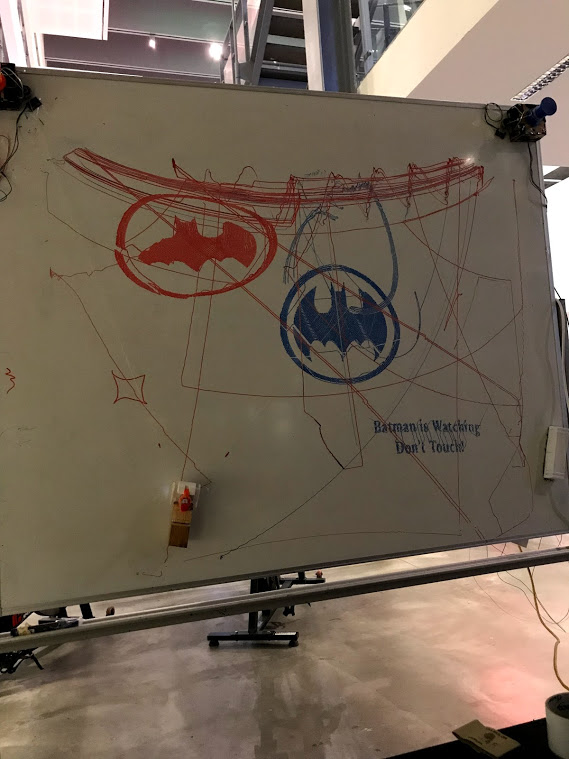
\includegraphics[scale=0.30]{Images/Jacobselskovsbilleder/IMG_2045.jpg}
\caption{ The Finale Canvas }
\label{LastCanvas}
\end{figure}